% Created 2025-07-05 Sat 15:19
% Intended LaTeX compiler: pdflatex
\documentclass[11pt]{article}
\usepackage[utf8]{inputenc}
\usepackage[T1]{fontenc}
\usepackage{graphicx}
\usepackage{longtable}
\usepackage{wrapfig}
\usepackage{rotating}
\usepackage[normalem]{ulem}
\usepackage{amsmath}
\usepackage{amssymb}
\usepackage{capt-of}
\usepackage{hyperref}
\usepackage{listings}
\usepackage{color}
\usepackage{amsmath}
\usepackage{array}
\usepackage[T1]{fontenc}
\usepackage{natbib}
\author{Anders Munch}
\date{\today}
\title{Make figures for article}
\begin{document}

\maketitle
\section{Setup and load data}
\label{sec:orge24a45c}
\section{Multi state illustration}
\label{sec:org6284f65}
\begin{lstlisting}[language=r,numbers=none]
library(prodlim)
library(here)
nTrans <- 3
stateLabels = c("Initial","Cause 1", "Cause 2", "Censored")
crHist <- Hist(time = 1:nTrans, event = list(from = rep("1", nTrans), to = stateLabels[-1]))
plot(crHist,stateLabels = stateLabels,arrowLabels = FALSE,
     tagBoxes = c(0,1,2,-1),
     box.width = 25) 
\end{lstlisting}

\begin{center}
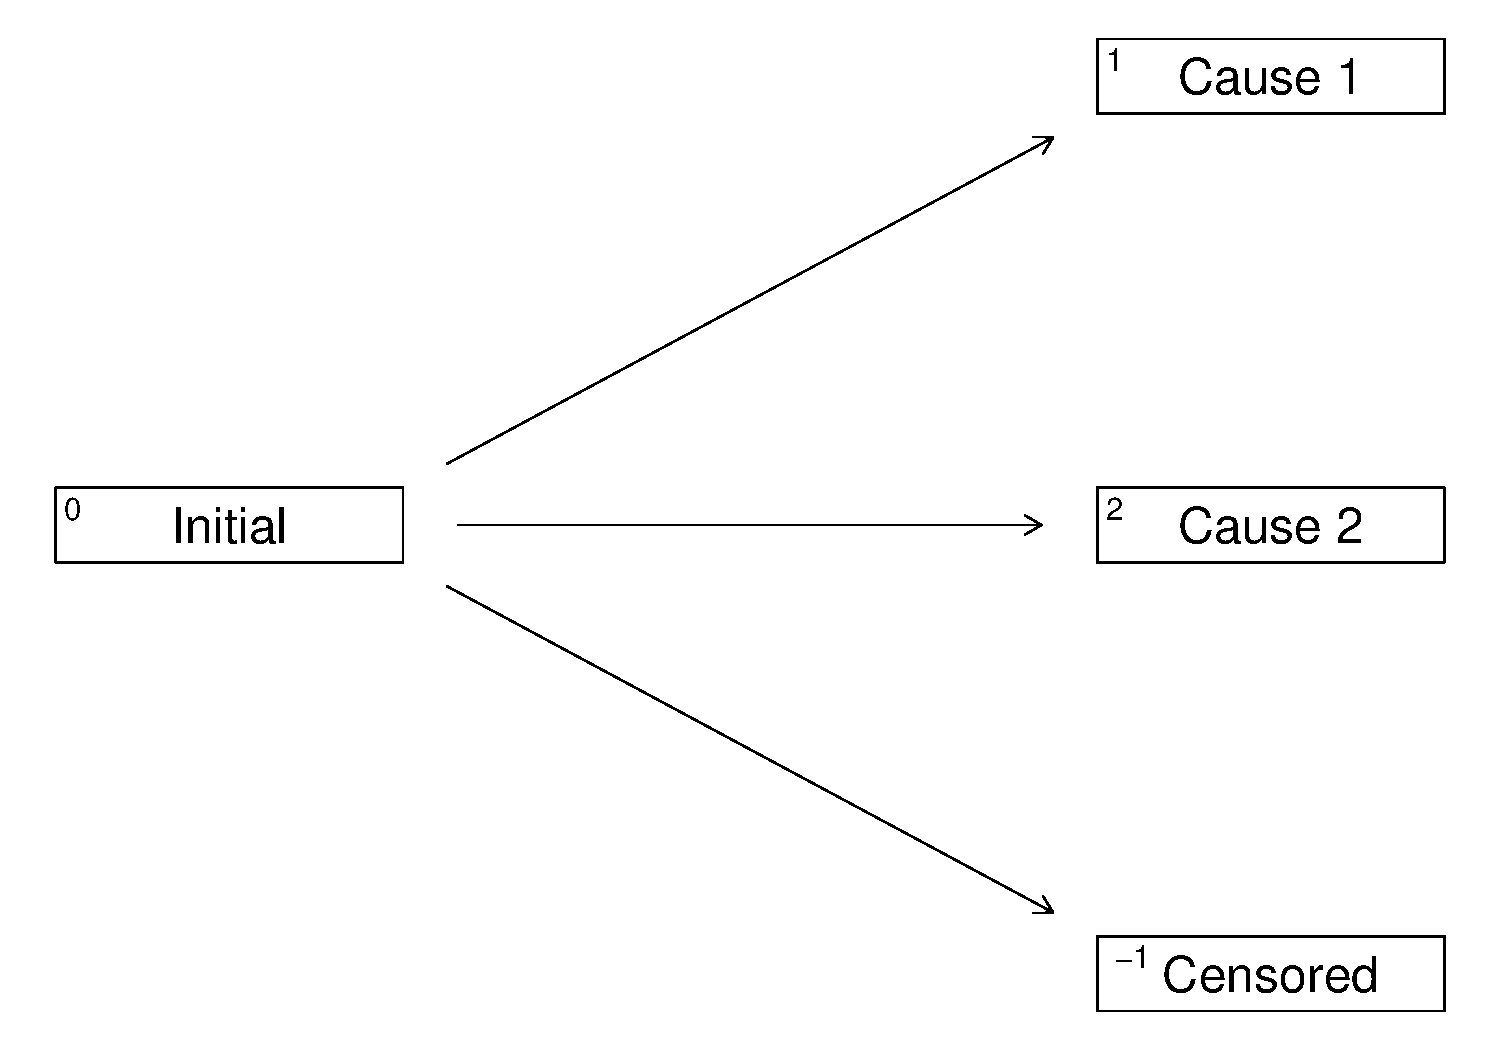
\includegraphics[width=.9\linewidth]{figure-multi-state-process.pdf}
\label{}
\end{center}
\section{Numerical experiments}
\label{sec:orgcfd1849}
Marginal event and censoring probabilities:
\phantomsection
\label{}
\begin{center}
\begin{tabular}{rlrrr}
time & sim\textsubscript{setting} & true\textsubscript{events} & true\textsubscript{cens} & at\textsubscript{risk}\\
\hline
36 & original & 24.619 & 61.853 & 25.774\\
36 & indep\textsubscript{cens} & 24.674 & 38.740 & 46.141\\
\end{tabular}
\end{center}
\subsection{IPCW based super learners}
\label{sec:org8486058}
\begin{lstlisting}[language=r,numbers=none]
  ipa_plot(data = summ_zel_sim2_1[time == 36 & type == "event" & SL != "survSL"])
\end{lstlisting}

\begin{center}
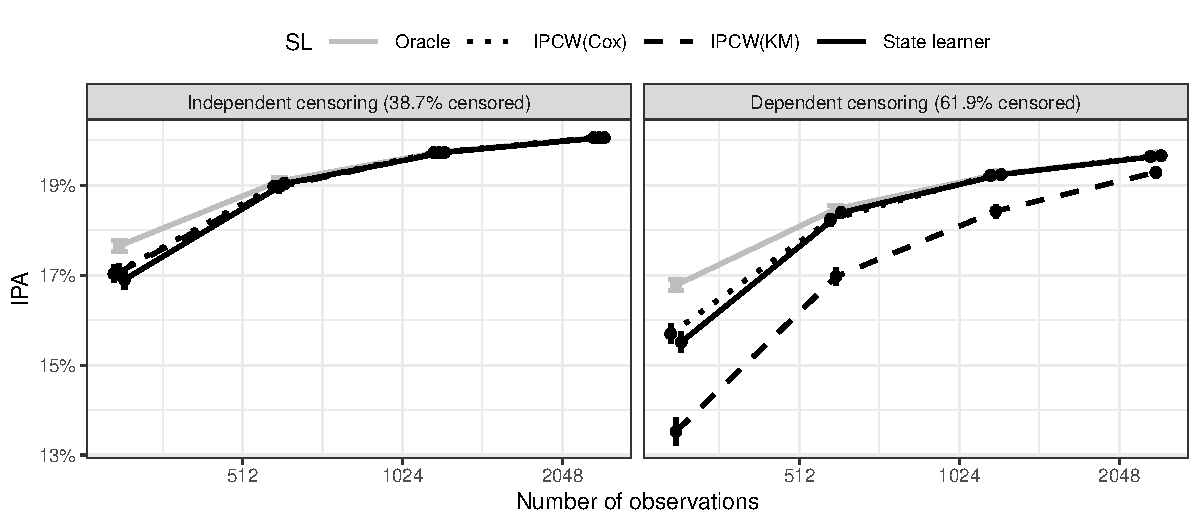
\includegraphics[width=.9\linewidth]{experiment-fig-sl-ipcw.pdf}
\label{}
\end{center}
\subsection{State learner versus survSL}
\label{sec:orgde73ddc}

\begin{lstlisting}[language=r,numbers=none]
  ipa_plot(data = summ_zel_sim2_1[time == 36 & type == "event" & !grepl("IPCW", SL)],
           linetype_vals = c(1,1,2))
\end{lstlisting}

\begin{center}
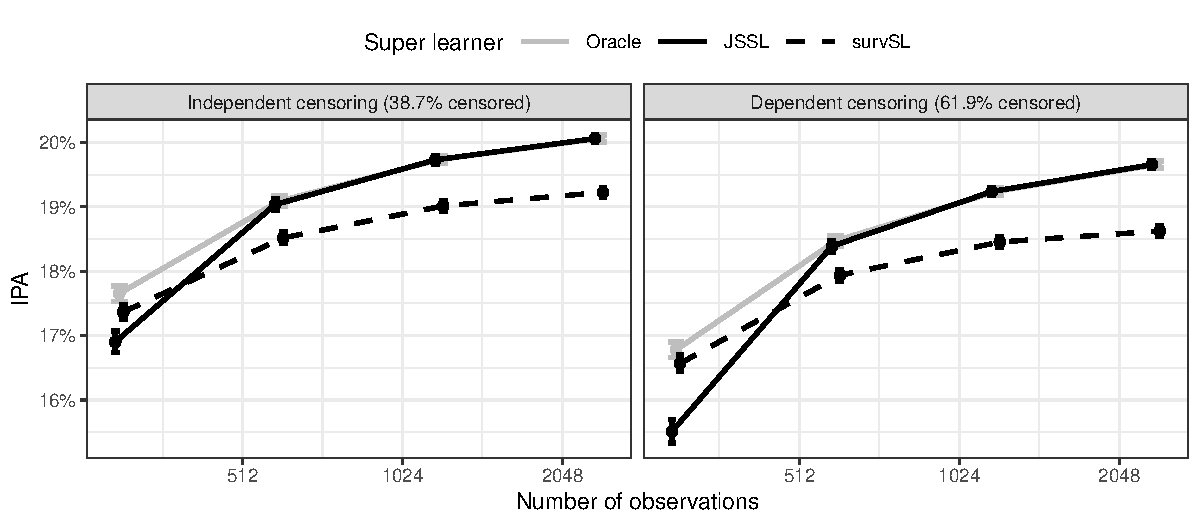
\includegraphics[width=.9\linewidth]{experiment-fig-sl-survSL-out.pdf}
\label{}
\end{center}

\begin{lstlisting}[language=r,numbers=none]
  ipa_plot(data = summ_zel_sim2_1[time == 36 & type == "cens" & !grepl("IPCW", SL)],
           linetype_vals = c(1,1,2), scales = "free_y", nrow = 2, ncol = 1)
\end{lstlisting}

\begin{center}
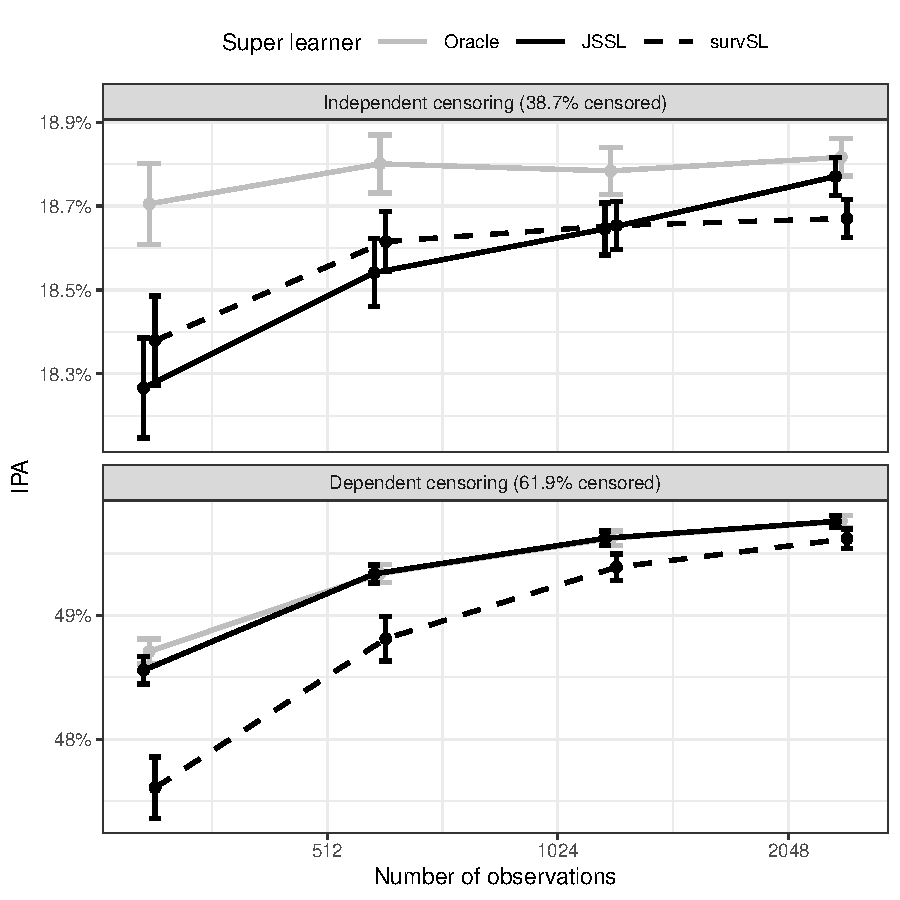
\includegraphics[width=.9\linewidth]{experiment-fig-sl-survSL-cens.pdf}
\label{}
\end{center}
\section{Data application with competing event}
\label{sec:orgeafe8e7}
\subsection{Table 1}
\label{sec:org89f8d1b}

\phantomsection
\label{}
\begin{verbatim}
\begin{tabular}{ l| c c c c c } 
 Rank&Cause 1&Cause 2&Censored&Loss&SD \\\hline
\hline
 $   1.0000 $&Elastic net&Elastic net&Random forest&$  7.0205 $&$ 0.030977 $ \\
\hline
 $   2.0000 $&LASSO&Elastic net&Random forest&$  7.0209 $&$ 0.031035 $ \\
\hline
 $   3.0000 $&Cox&Elastic net&Random forest&$  7.0224 $&$ 0.030871 $ \\
\hline
 $   4.0000 $&Elastic net&LASSO&Random forest&$  7.0225 $&$ 0.030170 $ \\
\hline
 $   5.0000 $&LASSO&LASSO&Random forest&$  7.0228 $&$ 0.030237 $ \\
\hline
 $  25.0000 $&Random forest&Random forest&LASSO&$  7.3845 $&$ 0.026975 $ \\
\hline
 $  50.0000 $&Elastic net&Random forest&LASSO&$  7.3974 $&$ 0.021290 $ \\
\hline
 $  75.0000 $&LASSO&Cox&LASSO&$  7.4059 $&$ 0.024660 $ \\
\hline
 $ 100.0000 $&Nelson-Aalen&Cox&Elastic net&$  7.8300 $&$ 0.016719 $ \\
\hline
 $ 125.0000 $&Nelson-Aalen&Nelson-Aalen&Nelson-Aalen&$ 10.3298 $&$ 0.003289 $ \\
\end{tabular}
\end{verbatim}




\begin{lstlisting}[language=r,numbers=none]
zel_real_plot_dt <- copy(zelefsky_statelearner$cv_fit)
learners_levels <- c("km","cox_unpenalized","cox_lasso","cox_elastic","rf")
learners_labels <- c("Nelson-Aalen","Cox","LASSO","Elastic net","Random forest")
zel_real_plot_dt[,cause1:=factor(cause1,levels=learners_levels,labels=learners_labels)]
zel_real_plot_dt[,cause2:=factor(cause2,levels=learners_levels,labels=learners_labels)]
## zel_real_plot_dt[,censor:=factor(censor,levels=learners_levels,labels=paste("Censoring learner\n", learners_labels))]
zel_real_plot_dt[,censor:=factor(censor,levels=learners_levels,labels=learners_labels)]
library(tidyverse)
df <- zel_real_plot_dt
df <- df[,label_wrapped:= str_wrap(paste(cause1,cause2,censor,collapse = ", "), width = 30)]

ggplot(df[cause2 == "Random forest"], aes(x = loss)) + geom_bar(stat="identity", position=position_dodge())+facet_grid(~cause1)

ggplot(zel_real_plot_dt, aes(x = cause1, y = cause2, fill = loss)) +
  geom_tile(color = "white") +
  facet_wrap(~censor) +
  scale_fill_viridis_c(option = "C") +
  labs(title = "Performance by Learner Combinations",
       x = "Cause 1 Learner", y = "Cause 2 Learner", fill = "Performance") +
  theme_minimal()

library(ggplot2)
ggplot(zel_real_plot_dt, aes(x = cause1, y = loss, col = cause2)) +
  geom_point(position=position_dodge(width=1), size=.8) +
  geom_errorbar(aes(ymin = loss-2*sd, ymax = loss+2*sd), width = .4,
                position=position_dodge(width=1)) +
  theme_bw() + ylab("Integrated Brier score") +
  theme(legend.position="top",
        axis.text.x = element_text(angle = 45, vjust = .8)) +
  xlab("Tumour learner") +
  facet_grid( ~ censor) +
  scale_colour_grey("Mortality learner", start = 0, end = 0.7)
\end{lstlisting}



\begin{lstlisting}[language=r,numbers=none]
zel_real_plot_dt <- copy(zelefsky_statelearner$cv_fit)
learners_levels <- c("km","cox_strata_stage","cox_lasso","cox_elastic","rf")
learners_labels <- c("N-Aa","Cox","lasso","elastic","RF")
zel_real_plot_dt[,cause1:=factor(cause1,levels=learners_levels,labels=learners_labels)]
zel_real_plot_dt[,cause2:=factor(cause2,levels=learners_levels,labels=learners_labels)]
zel_real_plot_dt[,censor:=factor(censor,levels=learners_levels,labels=paste("Censoring learner\n", learners_labels))]

library(ggplot2)
ggplot(zel_real_plot_dt, aes(x = cause1, y = loss, col = cause2)) +
  geom_point(position=position_dodge(width=1), size=.8) +
  geom_errorbar(aes(ymin = loss-2*sd, ymax = loss+2*sd), width = .4,
                position=position_dodge(width=1)) +
  theme_bw() + ylab("Integrated Brier score") +
  theme(legend.position="top",
        axis.text.x = element_text(angle = 45, vjust = .8)) +
  xlab("Tumour learner") +
  facet_grid( ~ censor) +
  scale_colour_grey("Mortality learner", start = 0, end = 0.7)
\end{lstlisting}

\begin{center}
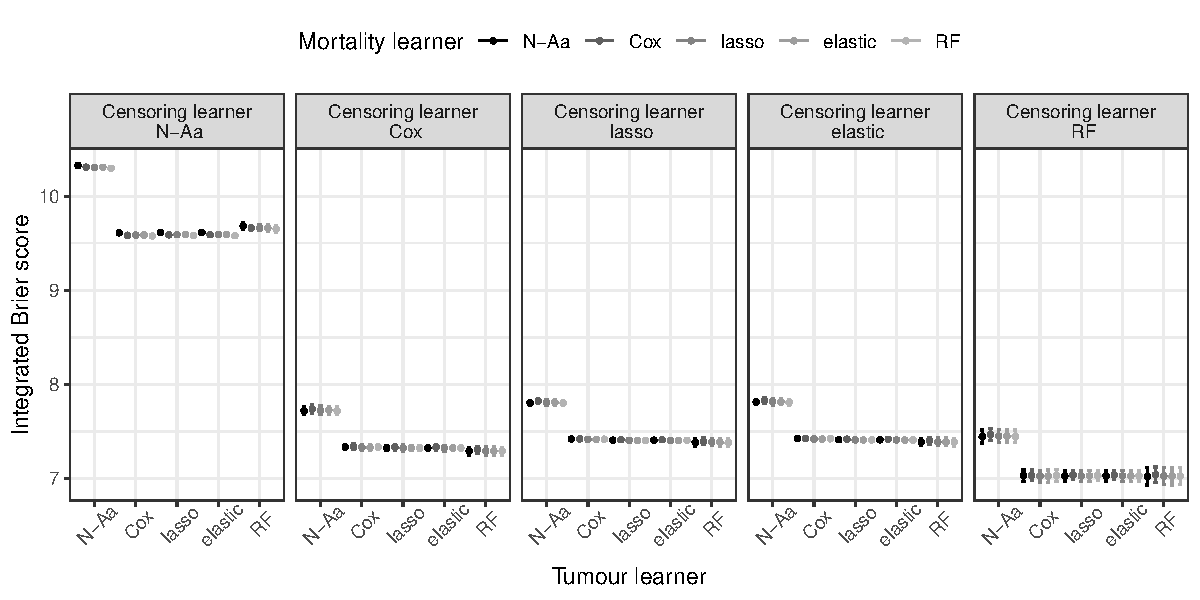
\includegraphics[width=.9\linewidth]{real-data-state-learner.pdf}
\label{}
\end{center}

Table
\subsection{Target parameter}
\label{sec:orge24e597}

\begin{lstlisting}[language=r,numbers=none]
  ate_est_inter_eff[effect == "ATE" & est_type == "one-step"] |>
    (\(plot_data)
      {
	plot_data[,cause:=factor(cause,levels=c("cause1","cause2"),labels=c("Tumor recurrence","Death"))]
	ggplot(plot_data, aes(x = time, y = est)) +
	  geom_errorbar(aes(ymin = lower, ymax = upper), width = 1) + 
	  geom_point() +
	  geom_hline(yintercept = 0, linetype = 2) +
	  theme_bw() +
	  facet_wrap( ~ cause) +
	  xlab("Months after baseline") + ylab("Average treatment effect of hormone therapy") +
	  scale_x_continuous(breaks = seq(6,36,12)) +
	  scale_y_continuous(labels = scales::percent)
      })()
\end{lstlisting}

\begin{center}
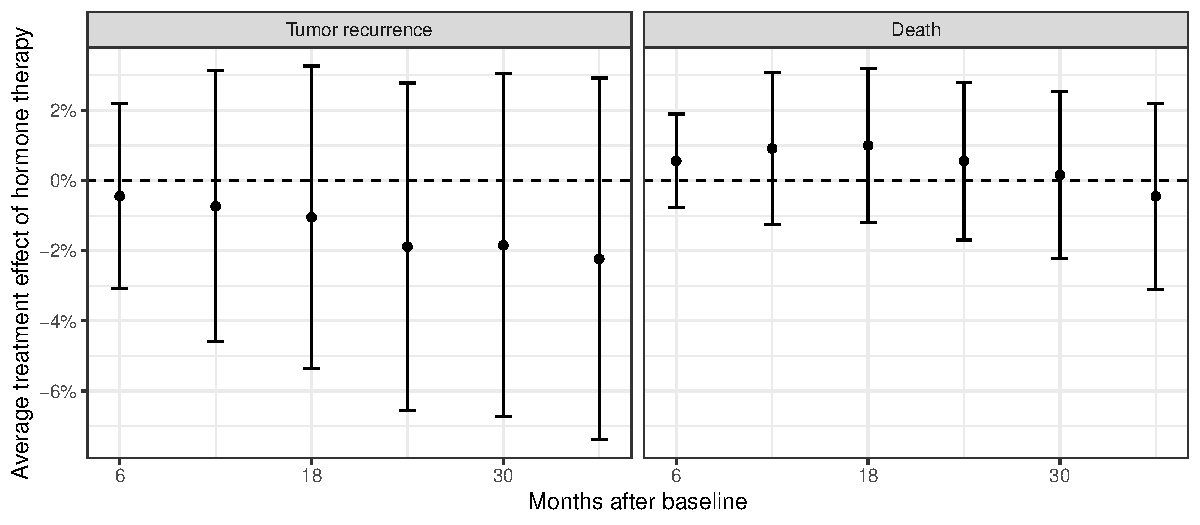
\includegraphics[width=.9\linewidth]{real-data-target.pdf}
\label{}
\end{center}
\end{document}
